\subsection{Entscheidungen}
\label{sub:entscheidungen}

  \subsubsection{Ideen}
  \label{ssub:ideen}
    Aus der Discover-Phase sind verschiedene Ideen entstanden. Zum Beispiel sah eine Idee vor, die interaktive Karte mit anderen Visualisierungsformen zu kombinieren. So könnten die einzelnen Trips auch als Balkendiagramm dargestellt werden. Diese könnten die zurückgelegte Strecke darstellen. Dabei war gedacht das man zwischen diesen verschiedenen Visualisierungsformen hin- und herschalten kann. Auch der Ansatz dies mit einer Tube-Map zu verbinden wurde als Idee notiert und war Zeitweise als mögliches Ziel definiert. 

  % subsubsection ideen (end)

    \subsubsection{Wahl der Datengrundlage}
  \label{ssub:wahl_der_datengrundlage}
    Im Abschnitt "`\nameref{ssub:einsatz_von_gps_daten}"' wurde bereits erklärt, wie der Einsatz von GPS-Daten eine Live Visualisierung ermöglichen könnte. Der Einstaz von GPS hat aber allerlei schwachstellen, die auf den ersten Blick vielleicht nicht offensichtlich sind.

    \begin{itemize}[label={}]
      \item \textbf{Fehlende Datenverfügbarkeit:}
        Ein Weg, um Echtzeitdaten zu visualisieren, wäre die Verarbeitung von GPS Daten, die von den jeweiligen Verkehrsverbünden zur Verfügung gestellt werden müssten. Dies ist allerdings nicht der Fall. Zwar gibt es durchaus eine Erfassung der öffentlichen Verkehrsmittel, allerdings werden diese nicht für Dritte zur Verfügung gestellt. Die HaCon GmbH sammelt beispielsweise solche Daten, indem sie diese durch in den Fahrzeugen integrierte Software berechnet.\parencite{havasBusradar}. Es wären also GPS Daten vorhanden, da sie unter anderem im Bus-Radar der Deutschen Bahn (entwickelt von HaCon) verwendet werden, sie sind allerdings weder über eine API noch anderweitig für die Öffentlichkeit erhältlich. Über die rechtlichen Belange und ob solche Daten in Deutschland überhaupt öffentlich gemacht werden dürften, soll an dieser Stelle nicht diskutiert werden\footnote{In \textit{"`Opening Public Transit Data in Germany"'} von Stefan Kaufmann\parencite{kaufmann} wird dieses Thema der Rechtslage näher betrachtet.}.

      \item \textbf{Aktualisierungsintervall:}
        Abseits der fehlenden Beschaffung von GPS Daten haben diese noch einen weiteren Nachteil. Vehicle, die mit einer GPS Lokalisierung ausgestattet sind, senden keinen kontinuierlichen Strom an Daten, sondern nur in einem gewissen Aktualisierungsintervall. Zwar preist HaCon seinen Busradar durch folgende Aussage an: 

        \begin{quote}
          \textit{"`Der neue Busradar eignet sich hervorragend, um die eigene Fahrt zu visualisieren und Anschlussfahrzeuge zu verfolgen. Erstmals geschieht dies GPS-basiert und nicht durch interpolierte Echtzeitdaten, was eine noch höhere Genauigkeit zur Folge hat."'}\parencite{havasBusradar}
        \end{quote}

        Nähme man aber nur die GPS Daten als Basis für eine Visualisierung, so würde der Bus bei jeder Aktualisierung von der jeweils vorherigen Position zur nächsten springen. Dieses "`Springen"' kann beim Busradar dann auch dazu führen, dass der Nutzer einen Bus auf seiner App verfolgen will, aber dieser nach dem nächsten GPS Update nicht mehr auf dem Display zu sehen ist, da er nun außerhalb des Viewports liegt. Dieses Verhalten kann den Nutzer durchaus verwirren, da nicht klar ist, in welche Richtung sich das Vehicle bewegt hat, sodass in alle Richtung gesucht werden muss.

      \item \textbf{Verlässlichkeit \& Verfügbarkeit:} 
        Zudem sind GPS Signale nicht immer verlässlich. Sie können oftmals gestört werden oder die Verbindung zum Satelliten verlieren. Wie würde sich in einem solchen Fall des Signalverlusts die Live Visualisierung verhalten? Verschwindet das Vehicle von der Karte oder bleibt es für längere Zeit auf der Stelle stehen? Beide Möglichkeiten erscheinen als nicht optimal. 

        Zuletzt sei erwähnt, dass ein GPS basiertes System für U- und S-Bahn erst gar nicht infrage käme, da diese unterirdisch verlaufen und andere Technologien für deren Erfassung eingesetzt werden müssten. Für eine Live Karte, die nicht nur Busse, sondern auch andere Verkehrsmittel abbilden möchte, ist die GPS basierte Lokalisierung folglich nicht zielführend.
    \end{itemize} 

    Wie zu sehen ist sind diese Probleme nicht unerheblich. Vor allem das fehlen der Daten, macht eine GPS basierte Visualisierung unmöglich.\\

    Aber auch GTFS besitzt Nachteile. Für eine Live Visualisierung fehlt ihr die Echtzeitkomponente. Die Fahrplandaten stellen nur einen \texttt{Soll-Zustand} dar, der erheblich vom \texttt{Ist-Zustand} abweichen kann. Auch die Geschwindigkeit eines Vehicles entspricht bei einer Interpolation der Durchschnittsgeschwindigkeit, die sich Anhand der Fahrplandaten ausrechnen lassen. Benötigt ein Vehicle $V$ von Station A nach B 3 Minuten für eine Strecke von 1.2 Kilometer, so würde die Animation eine durchschnittliche Geschwindigkeit von $v = \frac{s}{t} = \frac{1.2 \: \cdot \: 1000}{3 \: \cdot \: 60} = 6.6 \: \frac{m}{s} = 23.76 \: \frac{km}{h}$ errechnen.

    % TODO: sowas wie: "die Interpolation wird noch ausführlicher in Kapitel xy behandelt"

    Eine genauere Erfassung der Geschwindigkeit wäre zwar Wünschenswert, bringt allerdings andere Schwierigkeiten mit sich. Die Erfassung der Geschwindigkeit von jedem Vehicle würde eine hohe Menge an Daten bedeuten, die zwischen Server und Client ausgetauscht werden müssen. Ähnlich wie bei einer GPS basierten Animation, wäre der Client komplett davon abhängig, ständig Daten zu erhalten. Stelle man sich vor das mehrere hundert Anwender eine App benutzen wäre dies eine enorme Menge an Anfragen \& Antworten. Für Smartphones mit schlechter Verbindung ist dieser Umstand ein großes Problem. Ebenso wie die verwendete Bandbreite und der erhöhte Batterieverbrauch durch das ständige Stellen von Anfragen und der Verarbeitung der Antwort.

    Die Vorteile ergibt sich aus den eben genannten Nachteilen. Bei einer Interpolation des Fahrplans, ist keine ständige Verbindung zum Server nötig. Existiert der relevante Teil des Fahrplans auf dem Gerät des Endnutzers, so kann die Animation anhand dieser Daten erfolgen. Zudem wird das Problem des "`springens"' Umgangen, welches vor allem bei GPS basierter Animation ein Problem darstellt. Durch die Interpolation sind glatte Animationen der Vehicle auf der Karte möglich. Durch die Bewegung des Vehicles von A nach B entspricht die Visualisierung mehr dem Verhalten von Fahrzeugen in der realen Welt. Dadurch kann der Anwender besser nachvollziehen was geschieht.
    Eine Lösung für das Problem der fehlenden Echtzeiterfassung ließe sich GTFS-Realtime einsetzen. In dieser Arbeit kann GTFS-realtime allerdings nicht zum Einsatz kommen, da zum jetzigen Zeitpunkt\footnote{September, 2017}, der Verkehrsverbund Stuttgart-VVS dies nicht (auch nicht durch ein anderes Format) öffentlich anbietet.
    
  % subsubsection wahl_der_datengrundlage (end)

  \subsubsection{Gewählte Technologien}
  \label{ssub:gewählte_technologien}
    
    \subsubsection*{Datenbank}
    \label{ssub:datenbank}
      Da der GTFS Standard eine fertige relationale Beziehung der einzelnen Dateien festlegt, ist der Einsatz einer relationalen Datenbank sehr naheliegend. Dabei gibt es eine breite Palette an Auswahl. Damit die Anwendung möglichst Zugänglich bleibt, liegt der Fokus auf Datenbanken die unter einer Open-source Lizenz kostenfrei zur Verfügung stehen. Die zwei populärsten sind MySQL und PostgreSQL\parencite{db_engines}. Beide haben ihre Vor- und Nachteile und die Entscheidung ist mehr eine persönliche Präferenz, als ein großer Vorteil des Einen über den Anderen. Einen kleinen Vorteil bietet PostgreSQL's Unterstützung für Array-Types, welche sehr hilfreich beim Speichern und Abfragen von Daten ist. Ansonsten ist dieses Projekt auch mit MySQL realisierbar.
    % subsubsection datenbank (end)

    \subsubsection*{Kartenmaterial}
    \label{ssub:kartenmaterial}
      Bereits in Kapitel \ref{ssub:bewältigung_der_datenmenge} wurde die zu bewältigende Datenmenge angesprochen. Damit dies möglich ist wurde nach Software Lösungen gesucht, die für solche Datenmassen ausgelegt sind. Für die Karte wird dafür Mapbox eingesetzt. Mapbox verwendet Web-GL (basierend auf OpenGL) und bietet damit die Möglichkeit ein GPU unterstütztes Rendering im Browser zu ermöglichen. Zusätzlich bietet Mapbox gegenüber Google-Maps den Vorteil von eigene Karten-Styles. Diese können über Mapbox-Studio voll umfänglich auf die eigenen Bedürfnisse angepasst werden. Parks, Straßen, Schriftzüge, nahezu alle Elemente der Karte lassen sich ändern und anpassen. Zusätzlich können eigene Daten in die Karte integrieren werden, was Bandbreite und Rechenleistung spart. Damit konnten sämtliche Routen die das Stuttgart-VVS Feed beinhaltet, in das Kartenmaterial gezeichnet werden (siehe orangene Linien in Abbildung \ref{fig:map_tiles_routes}).

      \begin{figure}[htbp]
        \begin{center}
          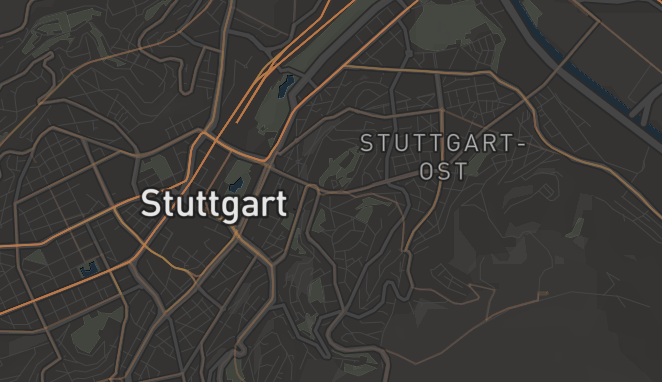
\includegraphics[width=0.5\textwidth]{map_tiles_routes}
          \caption{Karte mit integrierten Stuttgart-VVS Daten}
          \label{fig:map_tiles_routes}
        \end{center}
      \end{figure}
      
      Die Wahl der richtigen Tools ist dabei nur die Grundlage um die Datenmenge zu bewältigenden. Viele weitere Schritte sind notwendig um eine performante Webanwendung zu erstellen. Diese werden in Kapitel \ref{sub:backend} \nameref{sub:backend} und \ref{sub:frontend} \nameref{sub:frontend} ausführlich behandelt.

      % TODO: rework last paragraph
      
    % subsubsection kartenmaterial (end)
  % subsubsection gewählte_technologien (end)
% subsection entscheidungen (end)